%%%%%%%%%%%%%%%%%%%%%%%%%%%%%%%%%%%%%%%%%%%%%%%%%%%%%%%%%%%%%%%%%%
%%%%%%%%%%%%%%%%%%%%%%%%%%%%%%%%%%%%%%%%%%%%%%%%%%%%%%%%%%%%%%%%%%
%Packages
\documentclass[10pt, a4paper, french]{article}
\usepackage[top=3cm, bottom=4cm, left=3.5cm, right=3.5cm]{geometry}
\usepackage{amsmath,amsthm,amsfonts,amssymb,amscd, fancyhdr, color, comment, graphicx, environ}
\usepackage{float}
\usepackage{mathrsfs}
\usepackage[math-style=ISO]{unicode-math}
\setmathfont{TeX Gyre Termes Math}
\usepackage{lastpage}
\usepackage[dvipsnames]{xcolor}
\usepackage[framemethod=TikZ]{mdframed}
\usepackage{enumerate}
\usepackage[shortlabels]{enumitem}
\usepackage{fancyhdr}
\usepackage{indentfirst}
\usepackage{listings}
\usepackage{sectsty}
\usepackage{thmtools}
\usepackage{shadethm}
\usepackage{hyperref}
\usepackage{setspace}
\hypersetup{
    colorlinks=true,
    linkcolor=blue,
    filecolor=magenta,      
    urlcolor=blue,
}

\usepackage[francais]{babel}
\usepackage{datetime}  

\usepackage[T1]{fontenc}
\usepackage{lmodern}


%%%%%%%%%%%%%%%%%%%%%%%%%%%%%%%%%%%%%%%%%%%%%%%%%%%%%%%%%%%%%%%%%%
%%%%%%%%%%%%%%%%%%%%%%%%%%%%%%%%%%%%%%%%%%%%%%%%%%%%%%%%%%%%%%%%%%
%Environment setup
\mdfsetup{skipabove=\topskip,skipbelow=\topskip}
\newrobustcmd\ExampleText{%
An \textit{inhomogeneous linear} differential equation has the form
\begin{align}
L[v ] = f,
\end{align}
where $L$ is a linear differential operator, $v$ is the dependent
variable, and $f$ is a given non−zero function of the independent
variables alone.
}
\mdfdefinestyle{theoremstyle}{%
linecolor=black,linewidth=1pt,%
frametitlerule=true,%
frametitlebackgroundcolor=gray!20,
innertopmargin=\topskip,
}
\mdtheorem[style=theoremstyle]{Problem}{Problem}
\newenvironment{Solution}{\textbf{Solution.}}

\definecolor{codegreen}{rgb}{0,0.6,0}
\definecolor{codegray}{rgb}{0.5,0.5,0.5}
\definecolor{codepurple}{rgb}{0.58,0,0.82}
\definecolor{backcolour}{rgb}{0.95,0.95,0.92}

\usepackage{MnSymbol}

\lstdefinestyle{mystyle}{
    backgroundcolor=\color{backcolour},   
    commentstyle=\color{codegreen},
    keywordstyle=\color{magenta},
    numberstyle=\tiny\color{codegray},
    stringstyle=\color{codepurple},
    basicstyle=\ttfamily\footnotesize,
    breakatwhitespace=false,         
    breaklines=true,                 
    captionpos=b,                    
    keepspaces=true,                 
    numbers=left,                    
    numbersep=5pt,                  
    showspaces=false,                
    showstringspaces=false,
    showtabs=false,                  
    tabsize=2
}



\lstset{style=mystyle}
%%%%%%%%%%%%%%%%%%%%%%%%%%%%%%%%%%%%%%%%%%%%%%%%%%%%%%%%%%%%%%%%%%
%%%%%%%%%%%%%%%%%%%%%%%%%%%%%%%%%%%%%%%%%%%%%%%%%%%%%%%%%%%%%%%%%%
%Fill in the appropriate information below
\newcommand{\norm}[1]{\left\lVert#1\right\rVert}     
\newcommand\course{XXXX0000}                            % <-- course name   
\newcommand\hwnumber{0}                                 % <-- homework number
\newcommand\Information{Someone}                        % <-- personal information
%%%%%%%%%%%%%%%%%%%%%%%%%%%%%%%%%%%%%%%%%%%%%%%%%%%%%%%%%%%%%%%%%%
%%%%%%%%%%%%%%%%%%%%%%%%%%%%%%%%%%%%%%%%%%%%%%%%%%%%%%%%%%%%%%%%%%
%Page setup
\pagestyle{fancy}
\headheight 35pt
\lhead{\today}
\rhead{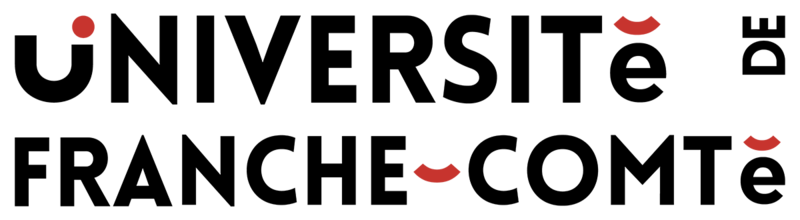
\includegraphics[width=2.5cm]{logo.png}}
\lfoot{}
\pagenumbering{arabic}
\cfoot{\small\thepage}
\rfoot{}
\headsep 1.2em
\renewcommand{\baselinestretch}{1.25}
%%%%%%%%%%%%%%%%%%%%%%%%%%%%%%%%%%%%%%%%%%%%%%%%%%%%%%%%%%%%%%%%%%
%%%%%%%%%%%%%%%%%%%%%%%%%%%%%%%%%%%%%%%%%%%%%%%%%%%%%%%%%%%%%%%%%%
%Add new commands here
\renewcommand{\labelenumi}{\alph{enumi})}
\newcommand{\Z}{\mathbb Z}
\newcommand{\R}{\mathbb R}
\newcommand{\Q}{\mathbb Q}
\newcommand{\NN}{\mathbb N}
\newcommand{\PP}{\mathbb P}
\DeclareMathOperator{\Mod}{Mod} 
\renewcommand\lstlistingname{Algorithm}
\renewcommand\lstlistlistingname{Algorithms}
\def\lstlistingautorefname{Alg.}
\newtheorem*{theorem}{Theorem}
\newtheorem*{lemma}{Lemma}
\newtheorem{case}{Case}
\newcommand{\assign}{:=}
\newcommand{\infixiff}{\text{ iff }}
\newcommand{\nobracket}{}
\newcommand{\backassign}{=:}
\newcommand{\tmmathbf}[1]{\ensuremath{\boldsymbol{#1}}}
\newcommand{\tmop}[1]{\ensuremath{\operatorname{#1}}}
\newcommand{\tmtextbf}[1]{\text{{\bfseries{#1}}}}
\newcommand{\tmtextit}[1]{\text{{\itshape{#1}}}}

\newenvironment{itemizedot}{\begin{itemize} \renewcommand{\labelitemi}{$\bullet$}\renewcommand{\labelitemii}{$\bullet$}\renewcommand{\labelitemiii}{$\bullet$}\renewcommand{\labelitemiv}{$\bullet$}}{\end{itemize}}
\catcode`\<=\active \def<{
\fontencoding{T1}\selectfont\symbol{60}\fontencoding{\encodingdefault}}
\catcode`\>=\active \def>{
\fontencoding{T1}\selectfont\symbol{62}\fontencoding{\encodingdefault}}
\catcode`\<=\active \def<{
\fontencoding{T1}\selectfont\symbol{60}\fontencoding{\encodingdefault}}

%%%%%%%%%%%%%%%%%%%%%%%%%%%%%%%%%%%%%%%%%%%%%%%%%%%%%%%%%%%%%%%%%%
%%%%%%%%%%%%%%%%%%%%%%%%%%%%%%%%%%%%%%%%%%%%%%%%%%%%%%%%%%%%%%%%%%
%Begin now!



\begin{document}

\begin{titlepage}
    \begin{center}
        \vspace*{3cm}
            
        \Huge
        \textbf{Projet Chrysalide}
            
        \vspace{1cm}
        \huge
        %Dorine Tabary
            
        \vspace{1.5cm}
        \Large
            
        %\textbf{\Information}                      % <-- author
        
            
        \vfill
                \vspace{1cm}
            
        %
\includegraphics[width=0.4\textwidth]{logo-hkust.png}
        
        \Large
        
        \today
            
    \end{center}
\end{titlepage}

%%%%%%%%%%%%%%%%%%%%%%%%%%%%%%%%%%%%%%%%%%%%%%%%%%%%%%%%%%%%%%%%%%
%%%%%%%%%%%%%%%%%%%%%%%%%%%%%%%%%%%%%%%%%%%%%%%%%%%%%%%%%%%%%%%%%%
%Start the assignment now
%%%%%%%%%%%%%%%%%%%%%%%%%%%%%%%%%%%%%%%%%%%%%%%%%%%%%%%%%%%%%%%%%%
%New problem
\newpage

\section{Résumé du projet (1 page maximum)}




%Le projet consiste à améliorer les connaissances en matière de quantique à travers l'étude d'un cas particulier qu'est le carré de Mermin. On énumèrera l'espace des solutions Formalisation de type combinatoire de la géométri quantique/symplectique. Nicolas Magaud



%Nous présentons des algorithmes et un code C pour décider de la contextualité quantique et évaluer le le degré de contextualité (une façon de quantifier la contextualité) pour une variété de géométries de lignes de points situées dans des espaces polaires symplectiques binaires de petit rang.  Avec ce code, nous avons pu non seulement de récupérer, de manière plus efficace, tous les résultats d'un article récent de Boutray et al (J. Phys. A : Math. Theor. 55 475301, 2022), mais nous sommes également parvenus à un certain nombre de nouveaux résultats dignes d'intérêt.
%L'article décrit d'abord les algorithmes et le code C. Il illustre ensuite sa puissance sur un ordinateur de poche. Il illustre ensuite sa puissance sur un certain nombre de sous-espaces symplectiques dont le rang varie de deux à sept. Les Les nouveaux résultats les plus intéressants sont les suivants (i) la non-contextualité des configurations dont les contextes sont des sous-espaces de dimension deux et plus, (ii) l'inexistence de sous-espaces négatifs de dimension trois et plus, (iii) l'existence de sous-espaces négatifs de dimension trois et plus. trois et plus, (iii) des bornes considérablement améliorées pour le degré de contextualité des quadriques elliptiques et hyperboliques pour les rangs quatre, ainsi que pour une sous-géométrie particulière de l'espace à trois qubit dont les contextes sont les lignes de cet espace, (iv) une preuve de la non-contextualité des perpsets et, enfin, mais pas seulement, une preuve de l'absence de contextualité de l'espace à trois qubits. perpsets et, enfin et surtout, (v) nature contextuelle d'une sous-géométrie distinguée d'une d'une nacelle multi-qubits, appelée two-spread, et le calcul de son degré de contextualité.

Dans le cadre de la mécanique classique, le résultat d'un calcul dépend des autres calculs effectués simultanément.
La mécanique quantique se distingue de ce modèle. En effet, un principe fondamental de la mécanique quantique repose sur la contextualité quantique. D'après le théorème de Kochen-Specker~\cite{RevModPhys.94.045007}, le résultat d'un calcul peut varier selon le contexte, ou plus précisément les autres calculs réalisés simultanément. La géométrie symplectique a été conceptualisée pour répondre à ces nouvelles contraintes. 

Le projet chrysalide a pour objectif d'améliorer la compréhension de la contextualité quantique.
% à travers l'analyse d'applications réduites modélisant la contextualité dans le traitement quantique de l'information.

Pour représenter le spin des particules quantiques, les matrices de Pauli forment une base de l'algèbre de Lie Symplectique~\cite{7110927}, avec

\begin{gather}
 \text{X}
 =
  \begin{pmatrix}
   $0$ & $1$ \\
   $1$ & $0$ 
   \end{pmatrix}, 
   \text{Y}
 =
  \begin{pmatrix}
   $0$ & $-i$ \\
   $i$ & $0$ 
   \end{pmatrix}, 
   \text{I}
 =
  \begin{pmatrix}
   $1$ & $0$ \\
   $0$ & $1$ 
   \end{pmatrix},
   \text{ et Z}=
  \begin{pmatrix}
   $1$ & $0$ \\
   $0$ & $-1$ 
   \end{pmatrix}
\end{gather}

Une première partie du projet s'intègre dans la thématique de la démonstration assistée par ordinateur.  Des résultats précédents~\cite{MULLER2022101853, contextAG}  ont mis en valeur des propriétés essentielles des espaces polaires symplectiques binaires et leur relation avec les groupes de Pauli généralisés de N-qubits. Ce projet a pour premier objectif de vérifier formellement les précédents résultats en implémentant un environnement déductif autorisant des calculs s'appuyant sur l'algèbre de Lie.
Les vérifications s'appuient sur des algorithmes pour générer des configurations quantiques et évaluer leur degré de contextualité.  

Une seconde partie a pour objectif de retrouver certains résultats préexistants~\cite{MULLER2022101853, contextAG} grâce à la programmation par contraintes ou la programmation logique, avec des possibilités d'amélioration à travers des calculs éventuellement plus rapides.

Une troisième partie a pour objectif d'améliorer le champs des connaissances à travers la génération et le comptage de structures issues d'un espace symplectique au nombre de q-bits limité, en tenant compte de la contextualité.

Une quatrième partie vise à lier les résultats de la théorie des groupes, à travers la recherche d'isomorphisme et d'invariant dans des structures géométriques réduites comme le carré de Mermin-Peres~\cite{mermin1993hidden}. Cette analyse a pour objectif de classer le groupe de symétrie de cette structure et de développer des nouvelles propriétés sur les carrés de Mermin-Peres. 



Une cinquième diversifie les travaux sur la contextualité quantique en appliquant les démarches de génération et de preuve au domaine des nombres de Raffalli~\cite{david2013asymptotically}. Un nombre de Raffalli est le nombre de possibilités de calculs à partir de fonctions prédéfinies composées de variables dont certaines sont libres. A partir du degré de liberté de ces variables, plusieurs combinaisons de fonctions sont possibles. Les nombres de Raffalli énumèrent ces combinaisons.


%Une cinquième partie élargit les travaux sur la contextualité quantique en appliquant les démarches précédentes au domaine des nombres de Raffalli~\cite{david2013asymptotically}. Un nombre de Raffalli est le nombre de possibilités de calculs à partir de fonctions prédéfinies composées de variables dont certaines sont libres. A partir du degré de liberté de ces variables, plusieurs combinaisons de fonctions sont possibles. Les nombres de Raffalli énumèrent ces combinaisons.

\newpage

\section{Projet scientifique (3 page maximum)}



\subsection{Etat de l'art}


%D'après l'article~\cite{holweck2021}, le développement d'ordinateurs quantiques nécessite de nouveaux outils pour réaliser des expériences quantiques à partir d'un ordinateur portable individuel. 
Les propriétés de la physique quantique, comme la contextualité, peuvent être traduites en expériences. Certaines de ces expériences peuvent être réalisables sur des ordinateurs quantiques. Cependant, la construction d'un ordinateur quantique universel sur lequel fonctionnerait n’importe quel algorithme et possédant un nombre significatif de qubits est soumis à de fortes contraintes.
La manipulation des qubits nécessite leur stabilité afin d'éviter que l'environnement les entourant ne modifie leur valeur par accident.
Dès lors, les ordinateurs quantiques sont fréquemment refroidis à des températures avoisinant le zéro absolu~\cite{holweck2021}.

Face à ces contraintes, l'objectif devient de modéliser avec une machine classique les différents états issus de la contextualité quantique. 
Les expériences sont réalisées avec des structures géométriques finies codant les relations de commutation du groupe de Pauli généralisé à N-qubits. Les limites prédites par les théories non contextuelles sont franchies, d'où la nécessité de fournir de nouvelles limites. 

Pour cela, le théorème de Kochen-Specker~\cite{RevModPhys.94.045007} permet de modéliser les différents états tenant compte de la contextualité en mécanique quantique.
 Ce théorème formalise que la mécanique quantique est en conflit avec les modèles classiques dans lesquels le résultat d'une mesure ne dépend pas des autres mesures compatibles effectuées conjointement.
Les mesures compatibles sont celles qui peuvent être effectuées simultanément ou, plus généralement, celles qui sont mesurables conjointement. Ce conflit est la contextualité quantique.
Dans cet article, une introduction à ce sujet et à son état actuel est présentée. Le théorème de Kochen-Specker est prouvé. Dans un second temps, plusieurs expérimentations sont réalisées, mettant en valeur les liens entre la contextualité et la non-contextualité. Enfin, certaines applications de la contextualité dans le traitement quantique de l'information sont examinées. 

Pour aller plus loin dans les connaissances en matière de contextualité, l'article~\cite{MULLER2022101853} s'intéresse à la géométrie symplectique, en proposant un algorithme générateur de structures selon le nombre de qubits. En plus de définir de nouvelles caractéristiques, une classification des structures générées est proposée, quand le nombre de qubits est égal à 4 ou 5.


Dans cette continuité, l'article~\cite{contextAG}
présente des algorithmes pour évaluer le degré de contextualité dans le cadre d'une variété de géométries dans des espaces polaires symplectiques binaires de petit rang. Les résultats sont présentés (i) la non-contextualité des configurations dont les contextes sont des sous-espaces de dimension deux et plus, (ii) l'inexistence de sous-espaces négatifs de dimension trois et plus, (iii) des bornes améliorées pour le degré de contextualité pour une configuration prédéfinie, (iv) une preuve de la non-contextualité des perpsets et (v) la nature contextuelle, et le calcul du degré de contextualité.

Parmi les modèles informatiques classiques développés depuis les travaux pionniers de Church et Turing, les modèles réalisables sont tous équivalents en termes de puissance de calcul.
Cependant, cette équivalence ne révèle rien sur le comportement interne les programmes. Les travaux sur les nombres de Raffalli s'intéressent à la question suivante :
A partir d'un langage de programmation théorique et d'une propriété, quelle est la probabilité qu'un programme aléatoire satisfasse la propriété donnée ? Le domaine des langages de programmation fonctionnels et, plus spécifiquement, le domaine du $\lambda$-calcul permettent de prendre en compte les propriétés syntaxiques dans cette analyse~\cite{david2009some}. Le projet chrysalide s'inscrit dans la continuité de ces précédents travaux en analysant les propriétés lors de calculs avec une ouverture préalablement définies.

\subsection{Objectifs}

Les objectifs de ce projet se situent dans la continuité des articles~\cite{contextAG} et~\cite{MULLER2022101853} avec :
\begin{enumerate}
    \item la vérification formelle de résultats précédents avec un assistant de preuve comme Coq~\cite{the_coq_development_team_2019_3476303} ou Why3~\cite{conf/esop/FilliatreP13}
    \item l'implémentation en Coq des constructions et des types afin d'autoriser les preuves dans un environnement basé sur la géométrie symplectique  
    \item l'implémentation en d'autres langages de programmation, en prolog et avec la programmation par contraintes (choco) afin de retrouver les résultats précédents (\cite{contextAG, MULLER2022101853})
    \item l'implémentation en ces autres langages de programmation de nouvelles méthodes éventuellement plus rapides/efficaces
    %\item la preuve de théorèmes générateurs, ou issus sur la recheche de groupes d'isomorphisme dans le cadre des carrés de Mermin-Peres
\end{enumerate}


\subsection{Résultats attendus}

Ce projet vise l'élargissement des connaissances en matière de géométrie quantique en :

\begin{itemize}
    \item reprenant des algorithmes précédents (\cite{contextAG, MULLER2022101853}) avec l'implémentation d'algorithmes dans d'autres langages, avec posssiblement des résultats plus rapides
    \item vérifiant formellement les propriétés précédentes (\cite{contextAG, MULLER2022101853})
    \item générer les structures en Coq permettant l'utilisation d'un environnement déductif dans le domaine de la géométrie symplectique
    \item amélioration des connaissances sur les carrés de Mermin-Peres, afin de faciliter la reconnaissance et la génération de cette structure
    \item amélioration de nos connaissances dans la thématique des nombres de Raffalli
    \item publications dans des conférences notamment CLA(Computational Logic and Applications) ou gandalf (Games, Automata, Logics, and Formal Verification), réalisation d'un exposé lors des séminaires VESONTIO.
\end{itemize}

\subsection{Expertise des participants dans le projet condidéré (références, bibliographie)}

Les travaux de l'équipe VESONTIO portent sur la qualité logicielle et améliore ou analyse la fiabilité, la sécurité ou la performance des systèmes à travers l'utilisation de plusieurs méthodes : la vérification ou preuve automatique. Dès lors, ce projet se situe dans la lignée directe de précédents travaux de l'équipe VESONTIO. Henry de Boutay~\cite{MULLER2022101853, de2022contextuality, contextAG} a permis l'analyse de propriétés de la géométrie symplectique. Axel Muller~\cite{MULLER2022101853, contextAG} a développé de nouveaux algorithmes dans ce domaine~\cite{MULLER2022101853, contextAG}. Pierre-Alain Masson lors de ces précédents travaux~\cite{de2022contextuality, de2021mermin} a pu apporter son expertise dans les calculs combinatoires. Alain Giorgetti~\cite{MULLER2022101853, de2022contextuality, contextAG, de2021mermin} a porté plusieurs projets dans ce domaine et a pu garantir à travers son expertise scientifique la rectitude de ces recherches, en plus du travail de réalisation et de validation de propriétés.

Mme Tabary peut apporter en plus des compétences dans le domaine de la complexité algorithmique, et de la classification de problèmes de décision, de comptage, d'énumération ou de génération, à l'instar de précédents travaux\cite{TomDavot}.

Un groupe de travail composé de Alain Giorgetti, Axel Muller, Pierre-Alain masson,  Dorine Tabary et Isabelle Jacques se réunit de façon hebdomadaire pour travailler sur ces thématiques.  




\newpage
\section{Mise en œuvre (2 pages max)}
\subsection{Principaux EC, chercheurs et doctorants impliqués dans le projet}

Les membres de l'équipe sont les suivants :
\begin{itemize}
    \item \textbf{Dorine Tabary}, maître de conférences en informatique, institut FEMTO-ST, Université de Franche-Comté, a travaillé dans le domaine de la complexité algorithmique
    \item \textbf{Alain Giorgetti}, maître de conférences en informatique, institut FEMTO-ST, Université de Franche-Comté, travaille dans les domaines de la vérification de programmes, des méthodes formelles et de la combinatoire
    \item \textbf{Axel Muller}, doctorant en informatique, institut FEMTO-ST, Université de Franche-Comté, travaille dans les domaines de la vérification de programmes, des méthodes formelles et de la combinatoire sous l'égide de Alain Giorgetti
    \item \textbf{Pierre-Alain Masson}, maître de conférences en informatique, institut FEMTO-ST, Université de Franche-Comté, travaille dans les domaines de la complexité et lde la programmation par contraintes
    \item \textbf{Nicolas Magaud}, maître de conférences en informatique, CNRS, université de Strasbourg, équipe Informatique Géométrique et Graphique, expert dans les logiciels d'assistance de preuve
    \item \textbf{Frédéric Holweck}, université de Technologie de Belfort-Montbéliard/Laboratoire Interdisciplinaire Carnot de Bourgogne, travaille dans le domaine de l'algèbre quantique
    \item \textbf{Metod Sanigi}, institut astronomique de Slovaquie, a travaillé dans le domaine de la géométrie quantique
\end{itemize}




\subsection{Méthodologie et choix des méthodes}

Ce projet nous amène dans un premier temps à vérifier formellement des algorithmes existants.
Dans un second temps, les bases de géométrie quantique sont implémentées afin de fournir un environnement de programmation propice aux vérifications des calculs issus de la géométrie symplectique.
La contextualité est ensuite analysée sur des exemples restreints avec un langage impératif de bas niveau et un langage logique. La vitesse de calculs est comparée avec d'autres résultats existants.


Les logiciels utilisés sont les suivants :
\begin{itemize}
    \item  Why3\footnote{\url{https://gitlab.inria.fr/why3/why3}}, plateforme de vérification déductive du premier ordre.
Cette plateforme est employée en raison de son utilisation intuitive.  Elle s'appuie sur des prouveurs de théorèmes externes, à la fois automatisés et interactifs, pour déterminer les conditions de vérification
    \item Coq\footnote{\url{https://coq.inria.fr/}}, assistant de preuve, doté d'un système de types dépendants d'ordre supérieur
    \item C\footnote{"\textit{The C programming language}", Brian W. Kernighan, Dennis M. Ritchie }, langage de programmation impératif, généraliste et de bas niveau
    \item Prolog\footnote{\url{https://www.swi-prolog.org/pldoc/doc_for?object=manual}}, langage de programmation logique
\end{itemize}





\subsection{Dépense prévisionnelle de la subvention}

Les dépenses sont les suivantes :
\begin{itemize}
    \item subvention d'un stagiaire de Master 2 : 3600 euros
    \item missions en Slovaquie : 1000 euros
\end{itemize}



\newpage


\section{Apport du projet (2 pages max)}
\subsection{Intégration dans la politique scientifique de l'université ou du laboratoire}


Les travaux de l'équipe VESONTIO portent sur la qualité logicielle et, améliore ou analyse la fiabilité, la sécurité ou la performance des systèmes à travers plusieurs grands domaines de recherche :
\begin{itemize}
	\item la modélisation formelle et semi-formelle en vue d'une analyse concentre des travaux autour de SysML et des systèmes composites
	\item l'étude de comment tester efficacement et automatiquement les systèmes
	\item la vérification ou preuve automatique 
\end{itemize} 

Ce projet s'intègre dans la troisième thématique de l'équipe \textbf{Vesontio} avec 
\begin{itemize}
    \item de la vérification formelle de résultats existants dans le domaine de la contextualité quantique
 \item  de la preuve automatique à travers l'implémentation des bases de la géométrie symplectique afin de permettre son utilisation dans toute preuve future
\end{itemize}

De plus, ce projet s'intègre directement dans la politique scientifique de l'Université de Franche-Comté qui vise à développer des projets pluri et transdisciplinaires. En effet, le projet proposé  se  situe au centre de trois grands domaines disciplinaires : les mathématiques avec l'utilisation de techniques combinatoires, l'informatique car les calculs s'appuient sur plusieurs logiciels que ce soit pour des preuves ou pour l'implémentation d'algorithmes, et la physique avec l'objectif central de ce projet qui consiste en l'amélioration des connaissances dans le domaine de la mécanique quantique.

\subsection{Apport ou plus-value locale/territoriale et/ou renforcement des coopérations de l'établissement}

En tant que nouvellement membre de l'équipe \textbf{Vesontio}, Mme Tabary peut apporter ses connaissances en complexité algorithmique afin de classer les types de problèmes rencontrés\cite{tabary2018new, TomDavot, tabary2020new}. 

L'équipe VESONTIO possède une grande expertise dans le domaine des vérifications formelles et de son application dans le domaine du quantique. Les travaux proposés s'intègrent directement dans la lignée de ces précédents travaux. 

De même, l'équipe VESONTIO est riche de plusieurs collaborations. Récemment, une collaboration avec M. Magaud, de l'Equipe Informatique Géométrique et Graphique du Département d'Informatique
Icube au CNRS, à l'Université de Strasbourg a permis d'utiliser et de développer les connaissances sur le logiciel Coq.
%%%%%%%%%%%%%%%%%%%%%%%%%%%%%%%%%%%%%%%%%%%%%%%%%%%%%%%%%%%%%%%%%%
%Complete the assignment now

\bibliography{biblio.bib}
\bibliographystyle{alpha-fr}

\end{document}

%%%%%%%%%%%%%%%%%%%%%%%%%%%%%%%%%%%%%%%%%%%%%%%%%%%%%%%%%%%%%%%%%%
%%%%%%%%%%%%%%%%%%%%%%%%%%%%%%%%%%%%%%%%%%%%%%%%%%%%%%%%%%%%%%%%%%
